\section{Question 1}
\subsection{Part a}
Satellite is in 600 km altitude circular orbit. Sun-synchronous orbit is desired. Find the inclination of the orbit.\\
\textbf{Solution:}\\
% np.arccos(-2/3*a**(7/2)*dOmega*(1-e**2)**2/(R**2*J2*np.sqrt(mu))) 
\begin{equation}
    i = \cos^{-1} \left(\dfrac{-2}{3} \dfrac{a^{7/2} \Delta \Omega (1-e^2)^2}{R^2 J_2 \sqrt{\mu}} \right) = \cos{-1} \left(\dfrac{-2}{3} \dfrac{(6978.14)^{7/2} 0.9856 (1-0.0000)^2}{(6398.14)^2 0.00108263 \sqrt{398600.4415}} \right) =\ang{97.788}
\end{equation}
\subsection{Part b}
Satellite is in 600 km altitude elliptical orbit.
 Sun-synchronous orbit is desired. Find the inclination of the orbit with e = 0.1.\\
\textbf{Solution:}\\
\begin{equation}
    i = \cos^{-1} \left(\dfrac{-2}{3} \dfrac{a^{7/2} \Delta \Omega (1-e^2)^2}{R^2 J_2 \sqrt{\mu}} \right) = \cos^{-1} \left(\dfrac{-2}{3} \dfrac{(6978.14)^{7/2} 0.9856 (1-0.1)^2}{(6398.14)^2 0.00108263 \sqrt{398600.4415}} \right) =\ang{97.632}
\end{equation}
\subsection{Part c}
Here is 3D chart indicating the relation between inclination, eccen-
tricity, and semi major axis of the orbit such that the orbit is Sun-Synchronous.
\begin{figure}[H]
    \centering
    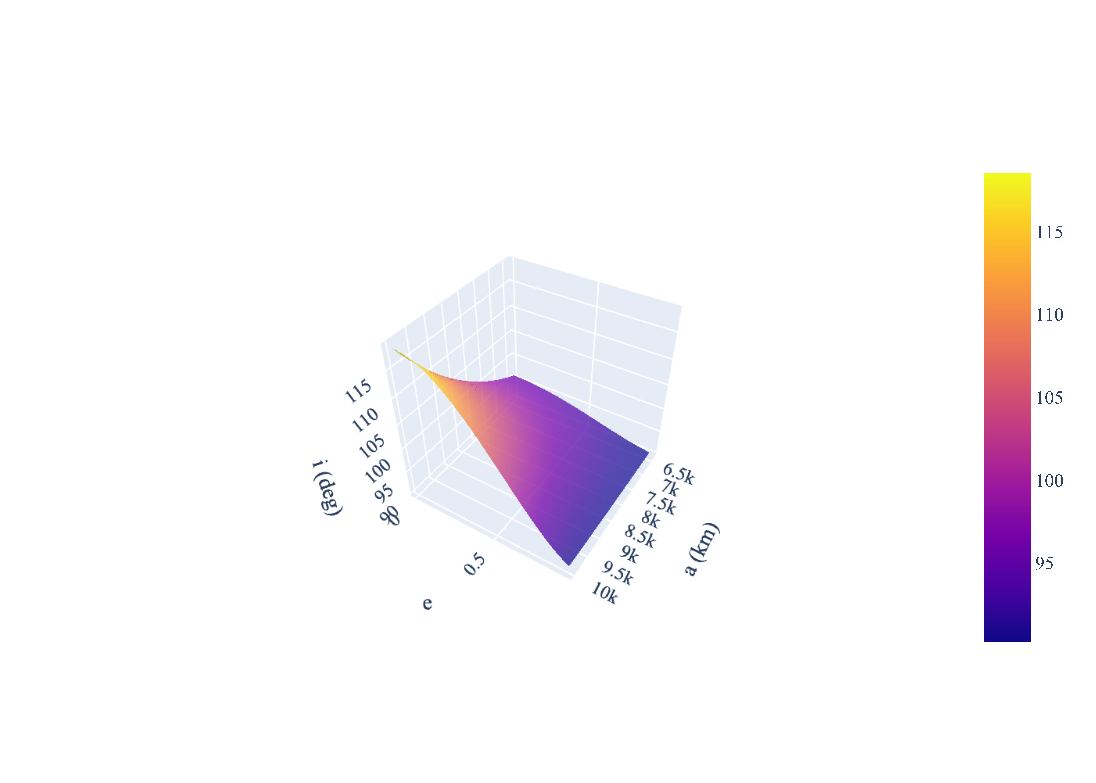
\includegraphics[width=\textwidth]{../Figure/Q1/3d_plot}
    \caption{3D plot of inclination, eccentricity and semi major axis}
\end{figure}
\subsection{Part d}
Here is the result for venus orbit.\\
\begin{figure}[H]
    \centering
    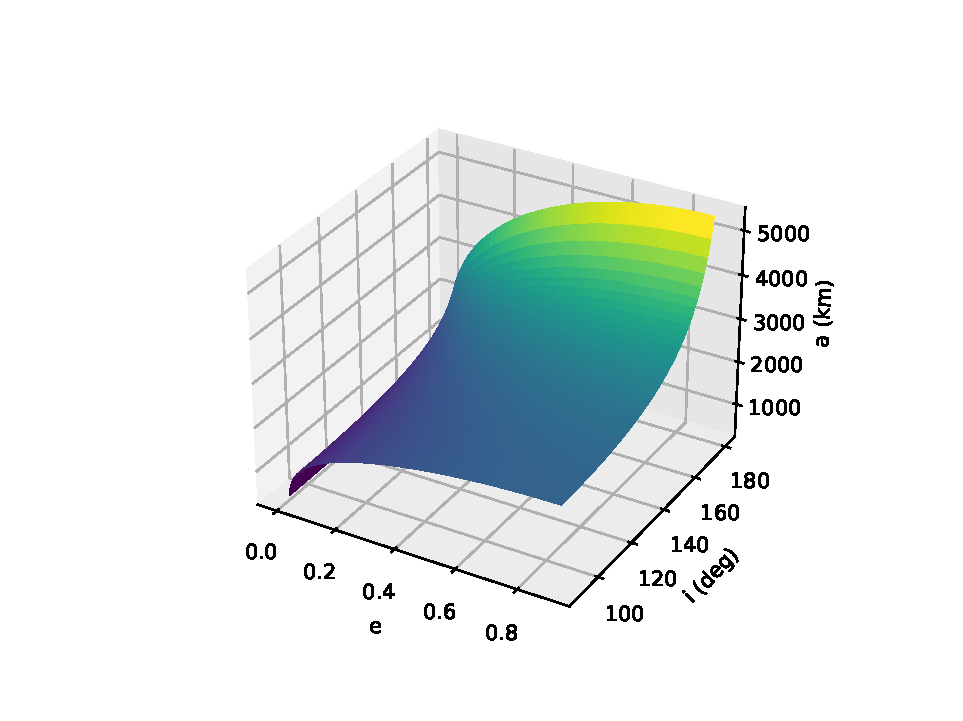
\includegraphics[width=\textwidth]{../Figure/Q1/Q1d_1}
    \caption{3D plot of inclination, eccentricity and semi major axis for venus}
\end{figure}
and here is result for pregee of orbits and venus orbit.
\begin{figure}[H]
    \centering
    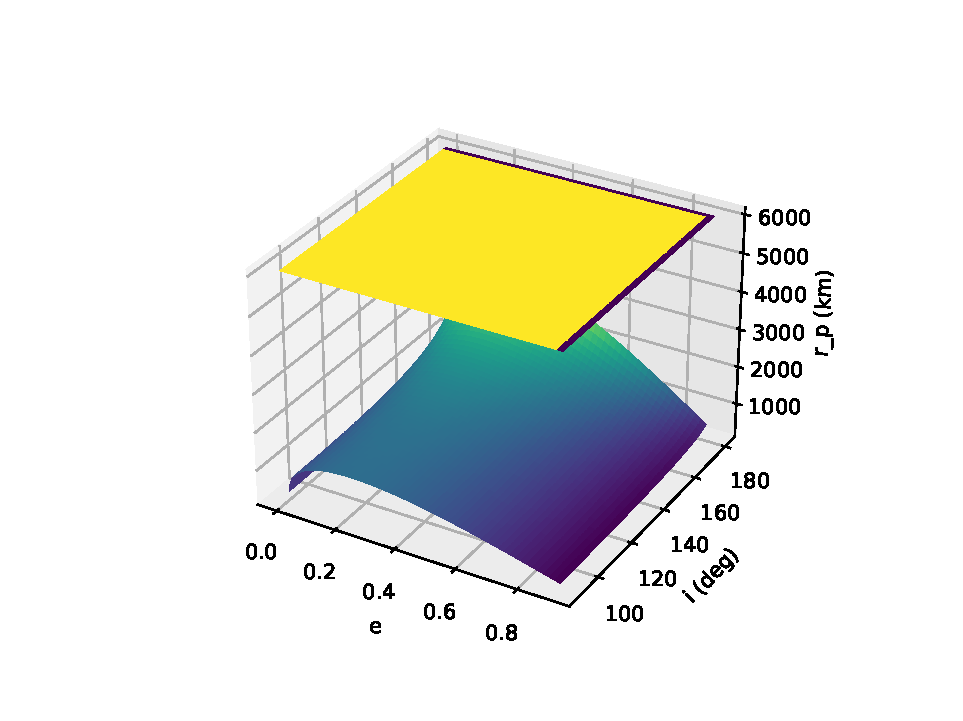
\includegraphics[width=\textwidth]{../Figure/Q1/Q1d_2}
    \caption{3D plot of inclination, eccentricity and perigee with venus radius surface}
\end{figure}
As we can see from above fig is that perigee of orbits are less than venus radius, so it is impossible to have sun-synchronous orbit around venus.
